\documentclass[12pt,a4paper]{article}
\usepackage{inverba, apacite}

\newcommand{\userName}{Cullyn Newman} 
\newcommand{\class}{PHL 316U} 
\newcommand{\theTitle}{Argumentative Meta-Analysis of Contemporary Liberal Democracy and Freedom}
\setlength\headheight{20pt}
\setlength{\parindent}{0pt}
\title{\hypertarget{home}\theTitle\vspace*{-0.4cm}}
\author{\normalsize\userName}
\date{\vspace*{-0.5cm}\small\today}
\renewcommand{\baselinestretch}{1.618} 

\usepackage{pgfplots}
\pgfplotsset{compat=newest}

\begin{document}

 
 
\usepgfplotslibrary{patchplots}
%%%%%%%%%%%%%%%%%%%%%%%%%%%%%%%%%%%%%%%%%%%%%%%%%%%%%%%%%%%%%%%%%%%%%
\maketitle
\begin{abstract}
\noindent In this essay I use a meta-analysis of mostly external references centered around the role of governance and its ability to promote genuine freedom. Heavy influences from a systems based thinking approach is used to emphasize the complexity of the problem. After establishing such complexities of the system we find ourselves in, I then move toward internal class readings in oder to critique and further the arguments made by David Harvey and Richard Sennett. I argue that the majority of both their arguments are very persuasive and cover significant areas of discussion. No concrete ideas regarding political reform sufficiently fullfil my desire for actionable change, but I argue both authors correctly direct attention towards areas in need of change.
\end{abstract}
\newpage
\fancyhead{}
\fancyhead[R]{\hyperlink{home}{\nouppercase\leftmark}}
\fancyhead[L]{\theTitle}
\rhead{\hyperlink{home}{\thepage}}%%%%%%%%%%%%%%%%%%%%%%%%%%%%%%%%%%%%%%%%%%%%%%%%%%%%%%%%

\subsubsection{Introduction}
\vspace*{-8pt}
The main focus of this essay involves the views of both David Harvey and Richard Sennett in regards to the dynamic interaction between contemporary liberal democracy and freedom of various scales. The arguments of both authors will eventually gravitate toward the center of the discussion, but the works of others will be included first in order to help establish the constraints on the increasingly complex interaction between governance and freedom. 

Overall, Harvey critiques are more broad, tackling the current state of neoliberalism and its relation to freedom, while Sennett critiques have an more indirect relation, as his focus is on work and culture and their roles in the complex system we find ourselves in. There is much to be discussed, so in this essay I start with an initial definition of system based thinking and then relate such mode of thought towards freedom and governance, which will then be used as a means to generate a more nuanced discussion designed to allow for more significant argumentative claims to be made on what society ought to strive for. Ultimately, I find most arguments by both authors very persuasive and support their positions; they tend to imply aspects contemporary democracy need to move away from the current neoliberal state in order to promote greater degrees of genuine freedom. 

\subsubsection{Thinking in Systems}
\vspace*{-8pt}
The initial urge when analyzing the works of Harvey and Sennett is to jump directly into the struggle between neoliberalism vs.\ socialism and their democratic impact on freedom of the people. This relationship between modes of governance stems from core disagreements mainly involving decentralization vs.\ centralization, free markets vs.\ regulation, and aristocracy vs.\ meritocracy, with of course other disagreements about maximization of profits, value of work, and more. 

Unfortunately, terms like democracy, socialism, and capitalism get thrown around far too often, resulting in such words being crude representations of various disagreements; confusion about such words often are the most significant barriers to productive discussion. Therefore, before I dive into an critiques of Harvey and Sennett, I will first establish the importance of system thinking as a means to reduce unproductive confusion due to our tendency to overly compress complex relationships. 

A fundamental observation about how most people tend to think was made apparent to me this year by a blog post made by Vitalik Buterin, a computer scientist, involving the differences in worldviews generalized into either a concave or convex representations. Other posts by him, and the book, \textit{Thinking in Systems: a Primer} by Donella H. Meadows and Diana Wright, have pushed me towards the adoption of system-like thinking that will be heavily used by me in this analysis. To help illustrate, here is a brief summary of Vatalik's work:


\begin{figure}[ht]

   \centering
   \caption*{{\color{neg}Convex} vs.\ {\color{liorange}Concave} Dispositions~\cite{vitalik}}
   \tikzset{every picture/.style={line width=0.75pt}}
   \scalebox{.75}{
   \begin{tikzpicture}[x=0.75pt,y=0.75pt,yscale=-1,xscale=1, color=darkText]  
      \draw  [color=neg,draw opacity=1 ][line width=1.5]  (32.11,108.37) .. controls (130.29,195.43) and (205.81,176.42) .. (258.67,51.33) ;
      \draw [line width=1.5]    (31.89,34.33) -- (31.89,186) ;
      \draw [shift={(31.89,30.33)}, rotate = 90] [line width=0.08]  [draw opacity=0] (13.4,-6.43) -- (0,0) -- (13.4,6.44) -- (8.9,0) -- cycle    ;
      \draw [line width=1.5]    (260.67,185) -- (31.89,185) ;
      \draw (31.89,194) node [anchor=north west][inner sep=0.75pt]   [align=left] {Option A};
      \draw (196,194) node [anchor=north west][inner sep=0.75pt]   [align=left] {Option B};
      \draw (110,194) node [anchor=north west][inner sep=0.75pt]   [align=left] {<< Policy >>};
      \draw (7,178) node [anchor=north west][inner sep=0.75pt]  [rotate=-270] [align=left] {Quality of Outcome};
   \end{tikzpicture}
      \hspace*{24pt}
   \begin{tikzpicture}[x=0.75pt,y=0.75pt,yscale=-1,xscale=1, color=darkText]
      \draw  [color=liorange, draw opacity=1 ][line width=1.5]  (576.4,166.63) ..controls (497.76,55.18) and (423.36,42.44) .. (353.2,128.4) ;
      \draw  [line width=1.5]    (352.89,37.33) -- (352.89,186) ;
      \draw [shift={(352.89,33.33)}, rotate = 90, color=darkText][line width=0.08] [draw opacity=0] (13.4,-6.43) -- (0,0) -- (13.4,6.44) -- (8.9,0) -- cycle    ;
      \draw [line width=1.5]    (577.67,185) -- (352.89,185) ;
      \draw (352.89,194) node [anchor=north west][inner sep=0.75pt]   [align=left]{Option A};
      \draw (517,194) node [anchor=north west][inner sep=0.75pt]   [align=left]{Option B};
      \draw (433,194) node [anchor=north west][inner sep=0.75pt]   [align=left] {<< Policy >>};
      \draw (320,178) node [anchor=north west][inner sep=0.75pt]  [rotate=-270][align=left] {Quality of Outcome};
   \end{tikzpicture}
   }          
\end{figure}

Essentially what this is describing is the tendency to gravitate toward the idea that one of two options is correct (convex), or that a combination tends to yield the best result (concave). Ironically, this dichotomy itself raises a meta concave and convex analysis about each philosophy. Taking a meta-concave approach: both are useful and each can have a greater degree of usefulness in terms of making useful predictions. However, elaborating on the superiority of such views is not why I bring this up. As Vitalik describes,

\begin{quotation}
   \color{G-Moon}
   \noindent ``Convex and concave are terms best suited to mathematical functions where the input and the output are both one-dimensional. The real world is high-dimensional---and as machine-learning researchers have now well established, in high-dimensional environments the most common setting that you can expect to find yourself in is not a universally convex or universally concave one, but rather a saddle point: a point where the local region is convex in some directions but concave in other directions.''~\cite{vitalik}
\end{quotation}

\begin{figure}[ht]
   \centering
   \caption*{Graphical Representation of a Saddle Point}
   \scalebox{.75}{
   \begin{tikzpicture}
      \begin{axis}
         \addplot3 [surf, draw=black,domain=-1.2:1.2,domain y=-1.5:1.5,opacity=0.6] {x^2-y^2};
      \end{axis}
   \end{tikzpicture}
   }
\end{figure}

As you add more dimensions, then the complex interaction between multiple concave and convex relationships produces local minima and maxima in the form of saddle points. Even with just three dimensions, one can see how compressing such views into one dimensional thinking can result in demonstrably false predictions involving the quality of outcome. What happens when we take on even more multidimensional political philosophies? Exponential increases in the difficulty of meaningful compressions of the diverse idea-spaces---something our minds certainly are not well are equipped to handle. This is where system-thinking comes into play,

\begin{quotation}
   \color{G-Moon}
   \noindent``There are no separate systems. The world is a continuum. Where to draw a boundary around a system depends on the purpose of the discussion. We can't impose our will on a system. We can listen to what the system tells us, and discover how its properties and our values can work together to bring forth something much better than could ever be produced by our will alone.''~\cite{systems}
\end{quotation}

``Where we draw the borders'' is the compression---we have to be careful when doing this as it's very easy to draw wrong conclusions, but vital, because we can't see the system as a whole. Listening involves the investigation and careful drawing of borders around local systems we can observe. This is a tremendous distinction that needs to be constantly reinforced since we suffer from a multitude of cognitive biases that interfere with our own relative views of reality. 

\subsubsection{The Complexities of Freedom and Democracy}
\vspace*{-8pt}

Hopefully the importance of just how complex the interaction between the ideas that generate the rules of the system we are in has been made clear. Again, the goal of this elaboration is to provide a means for more nuanced arguments to be applied to Harvey and Sennett's analysis on the relation between contemporary liberal democracy and freedom. I've purposely left their views out of the discussion so far, as I am working from an external to an internal approach to the ideas discussed in this class. The remainder of external references will be used now as a means to help define the space of various dimensions of freedom and democracy.

In 2019 Tom Scott, an educator and science communicator, gave a speech at The Royal Institution, a British organization devoted to scientific education and research, titled: \textit{There is No Algorithm for Truth}. In the speech hs describes the issues of science communication in the age of social media. The last portion of his speech was titled: \textit{Echo Chambers and Nazi Bars}, where he focused on online moderation---which is extremely relevant to the role of freedom in governance. Essentially what Tom Scott described was the extremes of a concave relationship. The Nazi Bars analogy describs a place where no moderation takes place:
\begin{quote}
   \color{G-Moon}``The inevitable conclusion of ``let anyone say anything'' is that the worst people, having finally found a place to let them in, start to drive out the more careful and cautious.''~\cite{tom}
\end{quote} 
Meanwhile, the Echo Chamber respresents the other side of the extreme with minimal freedom: 
\begin{quote}
   \color{G-Moon} ``Anyone with a dissenting opinion is shouted down by a large crowd all of whom support each other in their views, whether those views happen to coincide with reality or not.''~\cite{tom}
\end{quote}
Both these extremes tend to reinforce themselves if no action is taken---leading to radical group think in both scenarios. This distinction highlights a core problem in the relationship between governance and freedom. 

Every place of discussion, online or offline, must take a stance on where to draw the line. One would assume there is an ideal line to draw, but again, it's not that simple. This is just one dimension in the multidimensional space that is our culture---they aren't even really opposites, instead the degree to radicalization is also influenced by the concavity of how centralized/decentralized the place of discussion is, e.g., the more centralization there is, then the more likely radicalization of one form dominates based on where the line is drawn. Likewise, groups too small may lead to pockets of ungoverned radicalization that also hinder societal decision making. Therefore, I'd argue we want to find the ideal a saddle point between the small, more dynamic and heavily moderated groups, and the less strict, overarching centralized rules meant to make sure no groups get out of hand and start to negatively impact others.  

I will now turn my attention now to internal class references, adding more dimensions, and narrowing the discussion further. Our week seven and eight readings, particularly those of Bruno Bosteels in \textit{What is a People} and David Graeber in \textit{Direct Action}, explore some similar and some other important aspects near the saddle point of the complex landscape between freedom, democracy, and citizenship. First, Bosteels notes that some exclusion is necessary, 
\begin{quote}\color{G-Moon}
   ``Whichever way we designate those who are either not the people or other than the people, there is no way of circumnavigating the fact that, both historically and conceptually speaking, this category is constituted on the basis of a necessary exclusion.''~\cite{people}
\end{quote}
Bosteels is acknowledging the fact that not everyone is free to participate in what we call ``the people.'' If you don't kick the Nazis out of the bar, then they will drive out others. Some exclusion is necessary. However, we can't be too quick to judge, otherwise we get an echo chamber. Boosteels then brings up a excellent question regarding work of theory, 
\begin{quote}\color{G-Moon}
   ``Can the work of theory actually contribute to the sharpening of this political potential, rather than shielding itself in the irrefutable radicalism reserved for those rare ones who—standing on the sidelines or tracking down one crisis after the other as so many ambulance chasers—are uniquely capable of seeing through all the blind spots of contemporary politics, whether on the left or on the right?''~\cite{people}
\end{quote}
I will soon elaborate more on this, but for now I think it's important to claim that Sennett's views are strongly in favor of the affirmative answer to this question. Next, I must plant another seed, one in the form of a question raised by Graeber and that is important for later criticism of both Harvey and Sennett,
\begin{quote}\color{G-Moon}
   ``The great problem has been how to translate the flow of information into structures of collective decision making—since decision making is the one thing that is almost impossible to do on the Internet. Or, more precisely, the question is: when and on what level are structures of collective decision making required?''~\cite{direct}
\end{quote}
This is the one of most essential, if not the most essential, problem to be solved in regards to democracy and it's promotion of genuine freedom---it's asking where we ought to be in the multidimensional landscape we find ourselves in. Again, I will elaborate more on this later, but from what I've read it seems neither author sufficiently addressed this problem, though they do get close to it. 

\subsubsection{On Harvey and Sennett}
\vspace*{-8pt}
I can now begin to focus on the arguments made by Harvey and Sennett now that the discussion sufficiently narrowed. Most of Harvey writing gives a history on neoliberalism, which has a significant influence on contemporary liberal democracy. The following best summarizes his core argument:
\begin{quote}\color{G-Moon}
``We can, therefore, interpret neoliberalization either as a utopian project to realize a theoretical design for the reorganization of international capitalism or as a political project to re-establish the conditions for capital accumulation and to restore the power of economic elites. In what follows I shall argue that the second of these objectives has in practice dominated. Neoliberalization has not been very effective in  revitalizing global capital accumulation, but it has succeeded remarkably well in restoring, or in some instances (as in Russia and China) creating, the power of an economic elite.''~\cite{neo}
\end{quote}
Here I have to nearly fully agree with Harvey. I support the observation's he's made in \textit{A Brief History of Neoliberalism} and later in \textit{Seventeen Contradictions and the End of Capitalism}. In large part, he critiques contemporary democracy in, mostly in regards to work and allocation of profits and capital. One thing I think he could have done better was spend more time addressing the rationale behind free markets and other forces driving the adoption of neoliberalism. Opponents still stand behind the power of laissez-faire governance, citing the decrease in ``freedom'' regulation would have, which allows them to dismiss his arguments too easily.

In large part, I think the valuation of merit was a major driving factor of the adoption of neoliberalism. An example was he when giving support for how neoliberalism increased wealth inequality,
\begin{quote}\color{G-Moon}
   ``One substantial core of rising class power under 
neoliberalism lies, therefore, with the CEOs, the key 
operators on corporate boards, and the leaders in the 
financial, legal, and technical apparatuses that surround this 
inner sanctum of capitalist activity. The power of the actual 
owners of capital, the stockholders, has, however, been 
somewhat diminished unless they can gain a sufficiently 
large voting interest to affect corporate policy. Shareholders 
have on occasion been bilked of millions by the operations 
of the CEOs and their financial advisers.''~\cite{neo}
\end{quote}

Here I think he failed to see how merit may have actually been the more significant factor. The rise in CEO's income reflects how values of moral desert in success that are increased in free-market societies. I argue that a failure to address the luck in our success is a huge blind-spot in our democracy. It changes how we vote, what we think people deserve, what we do with our profits, how we treat those that fail, and much more. 

Now, I have to immediately address that free-markets are not bad---they are incredibly efficient at times and often vital. Furthermore, it may even appear that I value aristocracy when I critique merit. This is not the case. Again, the world is a continuum, increasingly complex, and this gradient is part of the system we find ourselves in. Meritocracy is not exactly the opposite of an aristocracy, similar to nazi bars and echo chambers, both can lead to radicalization. Harvey points out how such thing is happening in our current meritocratic neoliberal democracy:
\begin{quote}\color{G-Moon}
   ``While this disparate group of individuals embedded in the 
corporate, financial, trading, and developer worlds do not 
necessarily conspire as a class, and while there may be frequent 
tensions between them, they nevertheless possess a certain 
accordance of interests that generally recognizes the 
advantages (and now some of the dangers) to be derived from 
neoliberalization. They also possess, through organizations like 
the World Economic Forum at Davos, means of exchanging 
ideas and of consorting and consulting with political leaders. 
They exercise immense influence over global affairs and possess 
a freedom of action that no ordinary citizen possesses.''~\cite{neo}
\end{quote}
Much of criticism I have on Harvey's work is concilated in his later work where he addresses more of the contradictions inherent in capitalism and thus our contemporary democracy. There are two final quotes from Harvey (the first is actually from Terry Eagleton, but Harvey was commenting on it) that signal that he realizes the essential problem Graeber pointed out:
\begin{quote}\color{G-Moon}
   ``Once the shackles on human flourishing have been removed, then it is far harder to say what will happen. For men and women are then a lot more free to behave as they wish within the confines of their responsibility for one another. If they are able to spend more of their time in what we now call leisure activities rather than hard at work, their behavior becomes even harder to predict. I say “what we now call leisure” because if we really did use the resources accumulated by capitalism to release large numbers of people from work, then we would not call what they did instead leisure.''~\cite{neo}


   ``The class opposition between capital and labour is dissolved into
associated producers freely deciding on what, how and when they will
produce in collaboration with other associations regarding the
fulfillment of common social needs.''~\cite{con}
\end{quote}
In the former quote Harvey argues that true freedom is thoroughly unpredictable. This argument for the right for human flourishing despite the uncertainty it brings should be emphasized against proponents of neoliberalism that take free-markets too far. In the latter quote Harvey then claims what true freedom can do, and ought to be used for---collectively deciding when, where, and what to do in order to fulfill common social needs. In a way this gives a means to answer Grabers question, but it doesn't fully solve it. 

I purposely left Sennett's work for last. Mostly because he had less to say on the political side of freedom and democracy---even he admits it,
\begin{quote}\color{G-Moon}
``I recognize also that the least developed side of my argument concerns politics—Arendt’s domain, the domain of ``statecraft.'' Modern
pragmatism could be said to take on faith Jefferson’s belief that learning to work well is the foundation of citizenship.''~\cite{craft}
\end{quote}
However, as he points out, learning to work well might part of the foundation of citizenship. I do have to admit I initially had significant qualms with Sennett, such as his tendency to use illustrative anecdotes as reasoning or just his stylistic choice in language in general. But those issues aren't that bad and don't really subtract from the core argument he is making. Eventually I began to understand the grand evolution in culture he is striving for. Essentially, he is arguing for an change in culture in order to drive positive social change, one that values craftsmanship, which he defines as, ``the desire to do something well for its own sake.''~\cite{craft} Now, this may not seem relevant at first, but I do have to agree with him, this attitude is essential. Before I get more into why, I do have to point out a few concerns I have with some claims of his.
\begin{quote}\color{G-Moon}
   ``For all this, craftsmanship has a cardinal virtue missing in the new culture’s idealized worker, student, or citizen. It is commitment\ldots~Commitment entails closure, forgoing possibilities for the sake of concentrating on one thing.''~\cite{craft}
\end{quote}
Here I either disagree with him, or disagree with the scope he is implying. If he means commitment to one skill or thing in general, then I disagree. From what I can tell, the people of history that tend to make the greatest impact for the common good tend to be interested in a variety of things. Time and time again you see successful people pursuing many interests then borrowing skills from each area and applying them to others, which often seeds significant innovations. However, if he means the commitment to focusing on one thing temporarily in order to improve, then I completely agree. Spending the time to focus and push through difficulty is an essential skill in itself. Initially, I assumed it was the former, but now I think it's the latter. He references towards Linux (my current pastime involves building a custom OS starting from the base Linux kernel) and CAD as examples when writing about the repression of difficulty is what lead me to reconsider,
\begin{quote}\color{G-Moon}
   ``Whereas Linux is set up to discover problems, CAD is often used to hide them. The difference accounts for some of CAD’s commercial popularity; it can be used to repress difficulty.''~\cite{craft}
\end{quote}
What I now realize is that when I work on the complicated, and often poorly documented aspects of Linux, then it does require hours of significant commitment\ldots~and a desire to smash my head through the screen at times. I don't have to do this, my degree is in biology, but I do it because I want to learn about how computers work. This voluntary commitment to hard work and the liberty to do so contributes positively to my sense of well being. When I overcome such difficulties I can confidently say it generates the most durable states of well-being and happiness in my life. So despite my qualms with Sennett, I do have to say I am now very much persuaded by the importance of his idea for what culture ought to move towards.

Previously I mentioned that Sennett would favor the affirmative answer to the question Boosteels posed. I argue that Sennett would agree with the idea that a focus on theory would allow the sharpening of political potential. In Sennett's concluding chapter he claims that the development of craft can be applied toward craft in our relationship between people,
\begin{quote}\color{G-Moon}
   ``I’ve stressed the positive, open role 
routine and practicing play in the work of crafting physical 
things; so too do people need to practice their relations 
with one another, learn the skills of anticipation and 
revision in order to improve these relations.''~\cite{craft}
\end{quote}
I'd say then the work of theory and by developing a cultural attitude towards craftsmanship would make him argue in support of Boosteels question. He does also imply the this commitment would favor socialism, but then comments on values implicit in human culture,
\begin{quote}\color{G-Moon}
``But there are craft reasons to credit pragmatism’s faith in democracy; 
these lie in the capacities on which human beings draw to 
develop skills: the universality of play, the basic 
capabilities to specify, question, and open up. These are 
widely diffused among human beings rather than restricted 
to an elite.''~\cite{craft}
\end{quote}
Here, the capabilities Sennett mentions are what I think are at the core of genuine freedom and allow for an excellent place to conclude the core arguments addressed in this essay. Abilities of individuals to pursue interests and play, open up and share with each other freely, and question things around them are the skills needed to answer the essential question Graeber raised. We need craftsmanship, we need a departure from neoliberalism, we need the ability to be unpredictable, and we need to be able to collectively listen then decide  on what to do in the systems we find ourselves in despite the enormous difficulty present in doing so. 
\clearpage
\bibliographystyle{apacite}
\bibliography{citations.bib}
%\endgroup
\end{document}